\section{Exercise 2: Series Circuit Analysis}

\subsection{Objective}
The purpose of this exercise is to measure the voltage and current values of a circuit in which resistors are connected in series.

\subsection{Equipment}
\begin{itemize}
    \item Digital Multimeter (DMM)
    \item Resistors ($1k\Omega$, $4.3k\Omega$)
    \item Breadboard
    \item Power Supply
    \item Wires (Jumper Cables \& Crocodile Clips)
\end{itemize}

\newpage
\thispagestyle{plain}

\subsection{Procedure}
\begin{enumerate}
    \item We have made the circuit analysis using LTspice and these are the results:
    \begin{figure}[h]
        \centering
        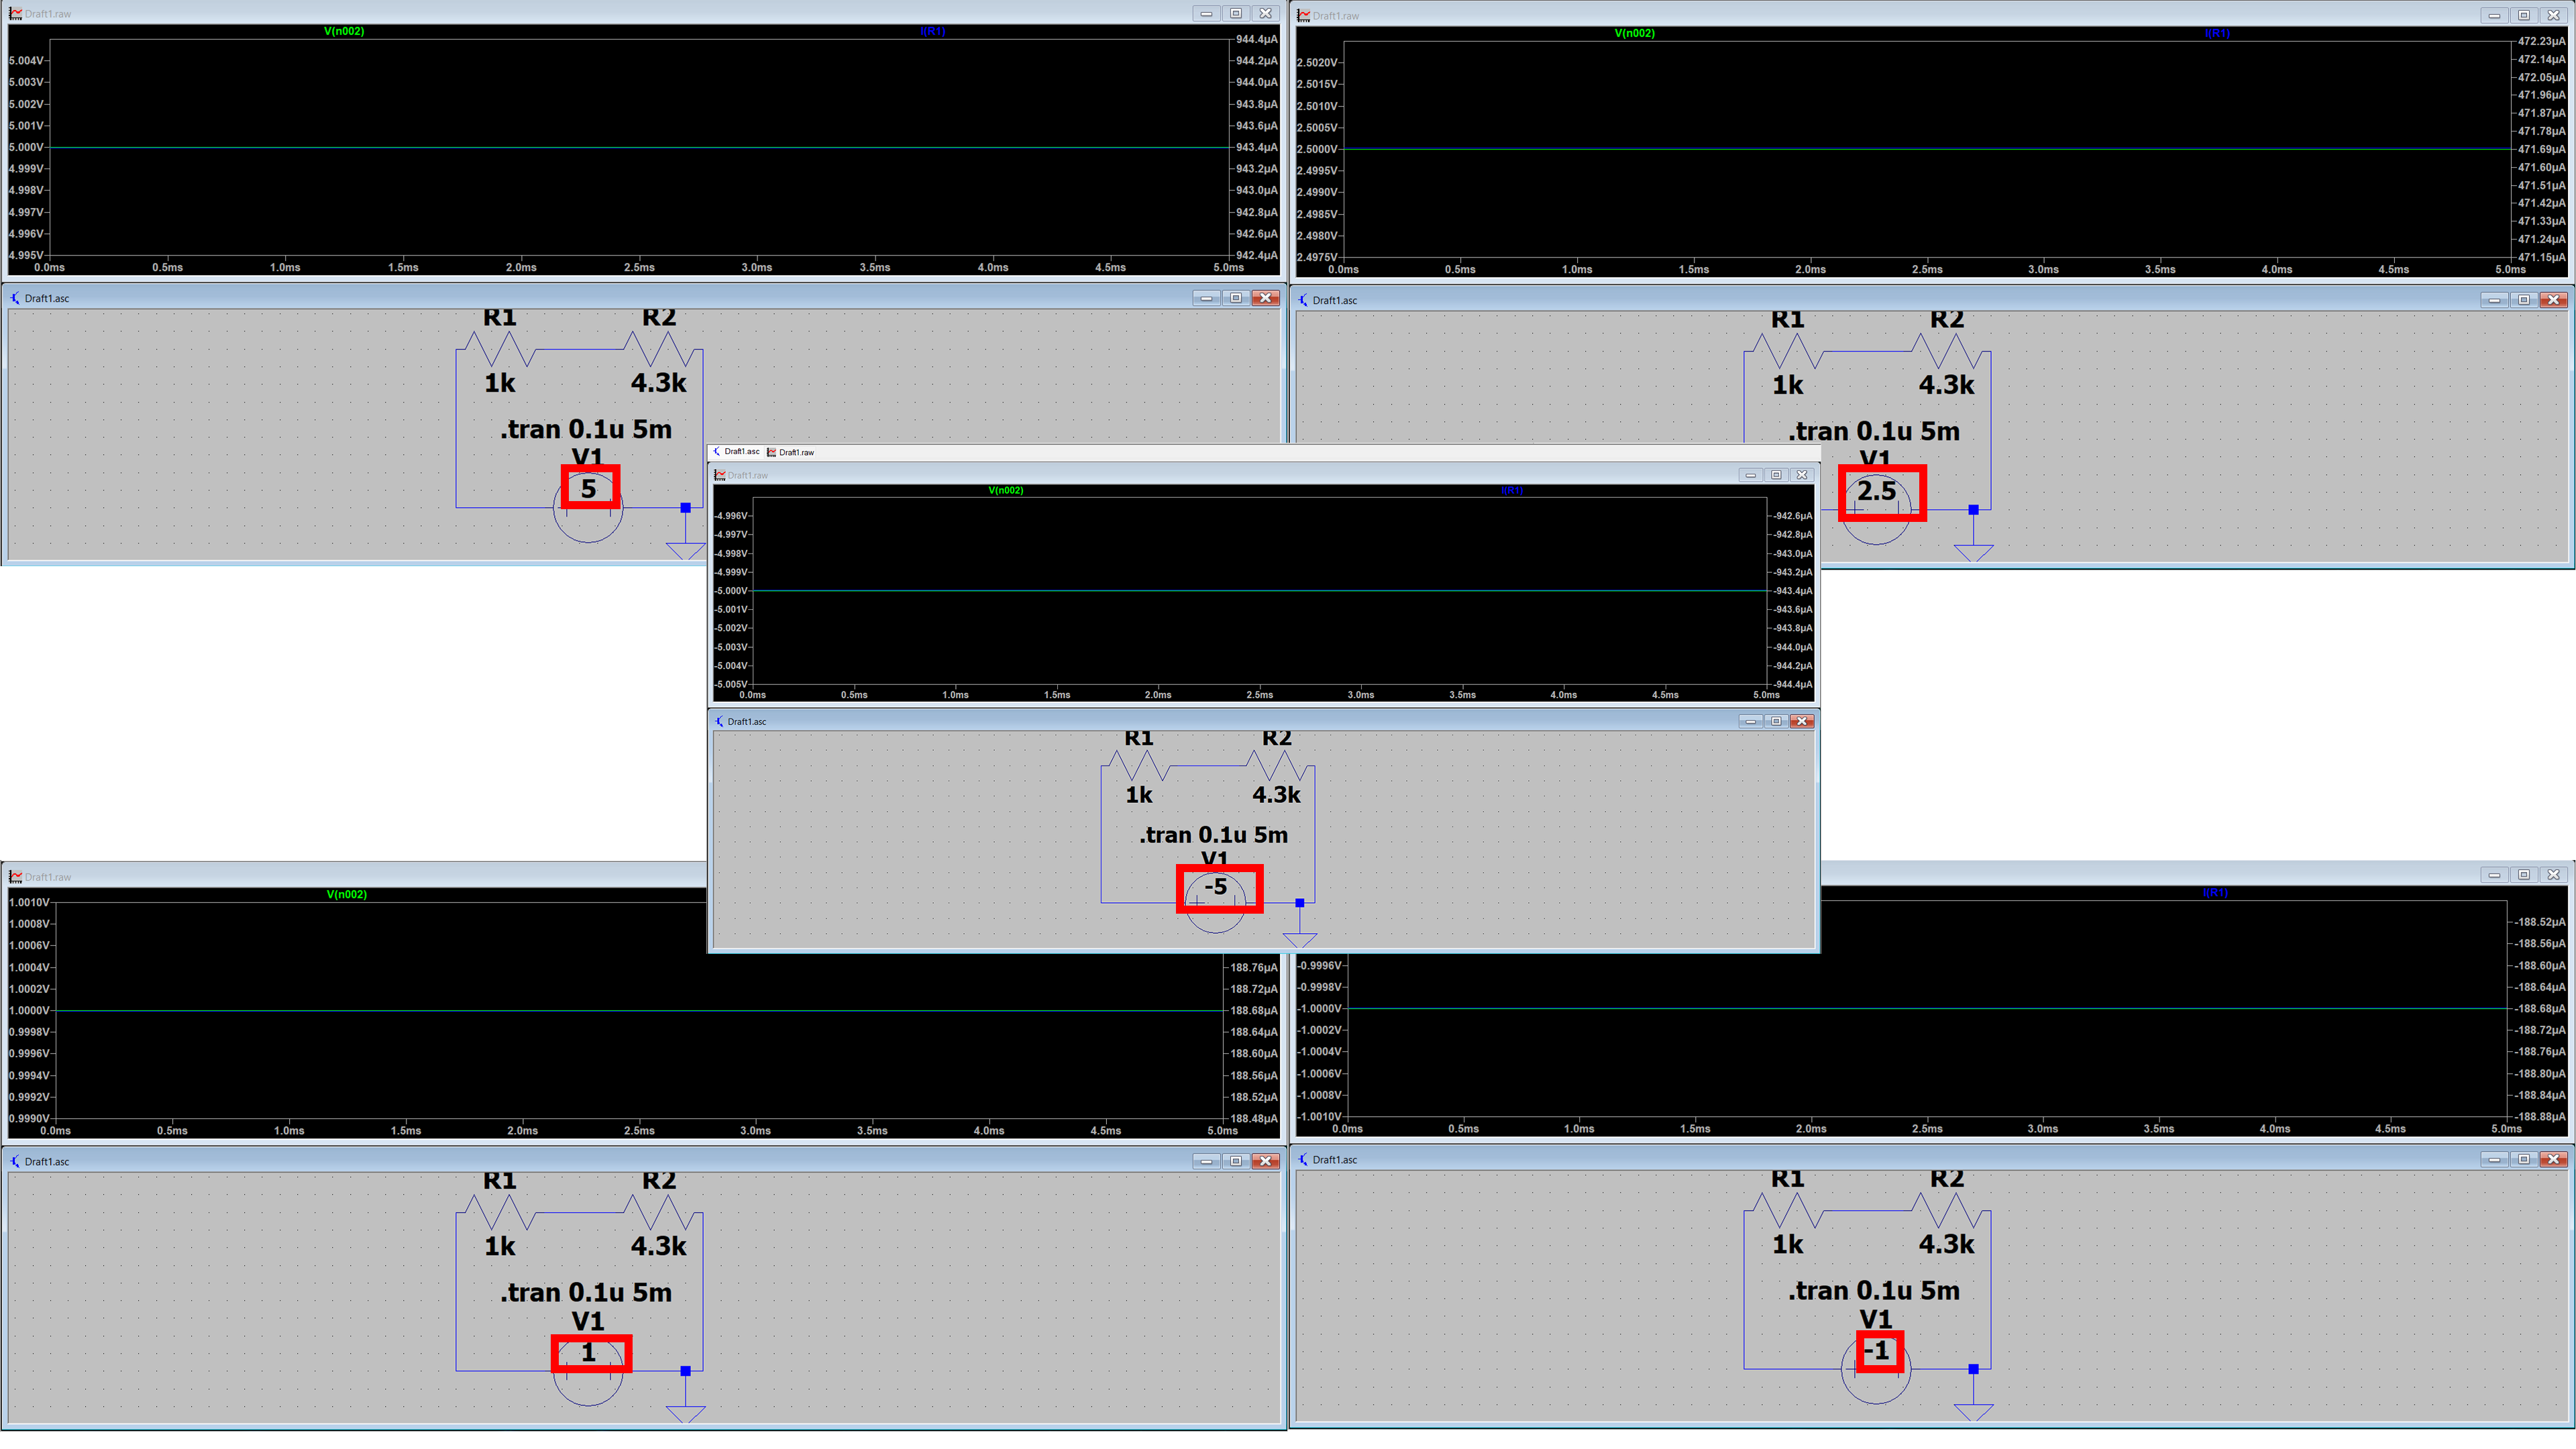
\includegraphics[width=1\textwidth]{assets/taks_2.png}
        \caption{Circuit Diagram \& Calculations}
    \end{figure}

    \begin{figure}[h]
        \centering
        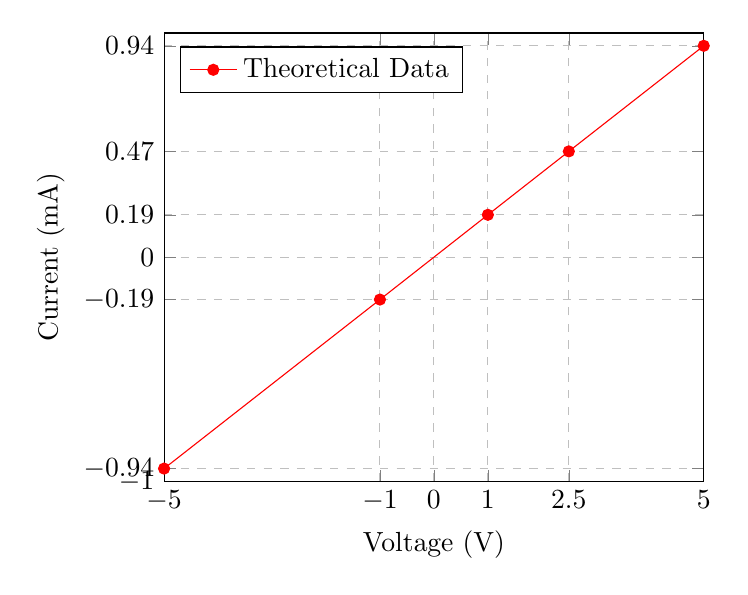
\begin{tikzpicture}
            \begin{axis}[
                xlabel={Voltage (V)},
                ylabel={Current (mA)},
                xmin=-5, xmax=5,
                ymin=-1, ymax=1,
                xtick={-5,-1,0,1,2.5,5},
                ytick={-1, -0.943, -0.189,0, 0.189, 0.472, 0.943},
                legend pos=north west,
                ymajorgrids=true,
                xmajorgrids=true,
                grid style=dashed,
            ]
                \addplot[
                    color=red,
                    mark=*,
                ]
                coordinates {
                    (-5, -0.943)
                    (-1, -0.189)
                    (1, 0.189)
                    (2.5, 0.472)
                    (5, 0.943)
                };
                \legend{Theoretical Data}
            \end{axis}
        \end{tikzpicture}
        \caption{Voltage-Current Graph of the Theoretical Circuit}
    \end{figure}

    \newpage
    \thispagestyle{plain}

    \item We have connected the resistors in series on the breadboard as shown in the figure below:
    \begin{figure}[h]
        \centering
        \begin{circuitikz} \draw
            (0, 7) to[battery] (0, 0)
            (0, 7) to[R, l=$1k\Omega$] (7, 7)
            (7, 7) to[R, l=$4.3k\Omega$] (7, 0)
            -- (0, 0);
        \end{circuitikz}
        \caption{Series Circuit with Two Resistors}
    \end{figure}
    \begin{figure}[h]
        \centering
        \begin{minipage}{.5\textwidth}
            \centering
            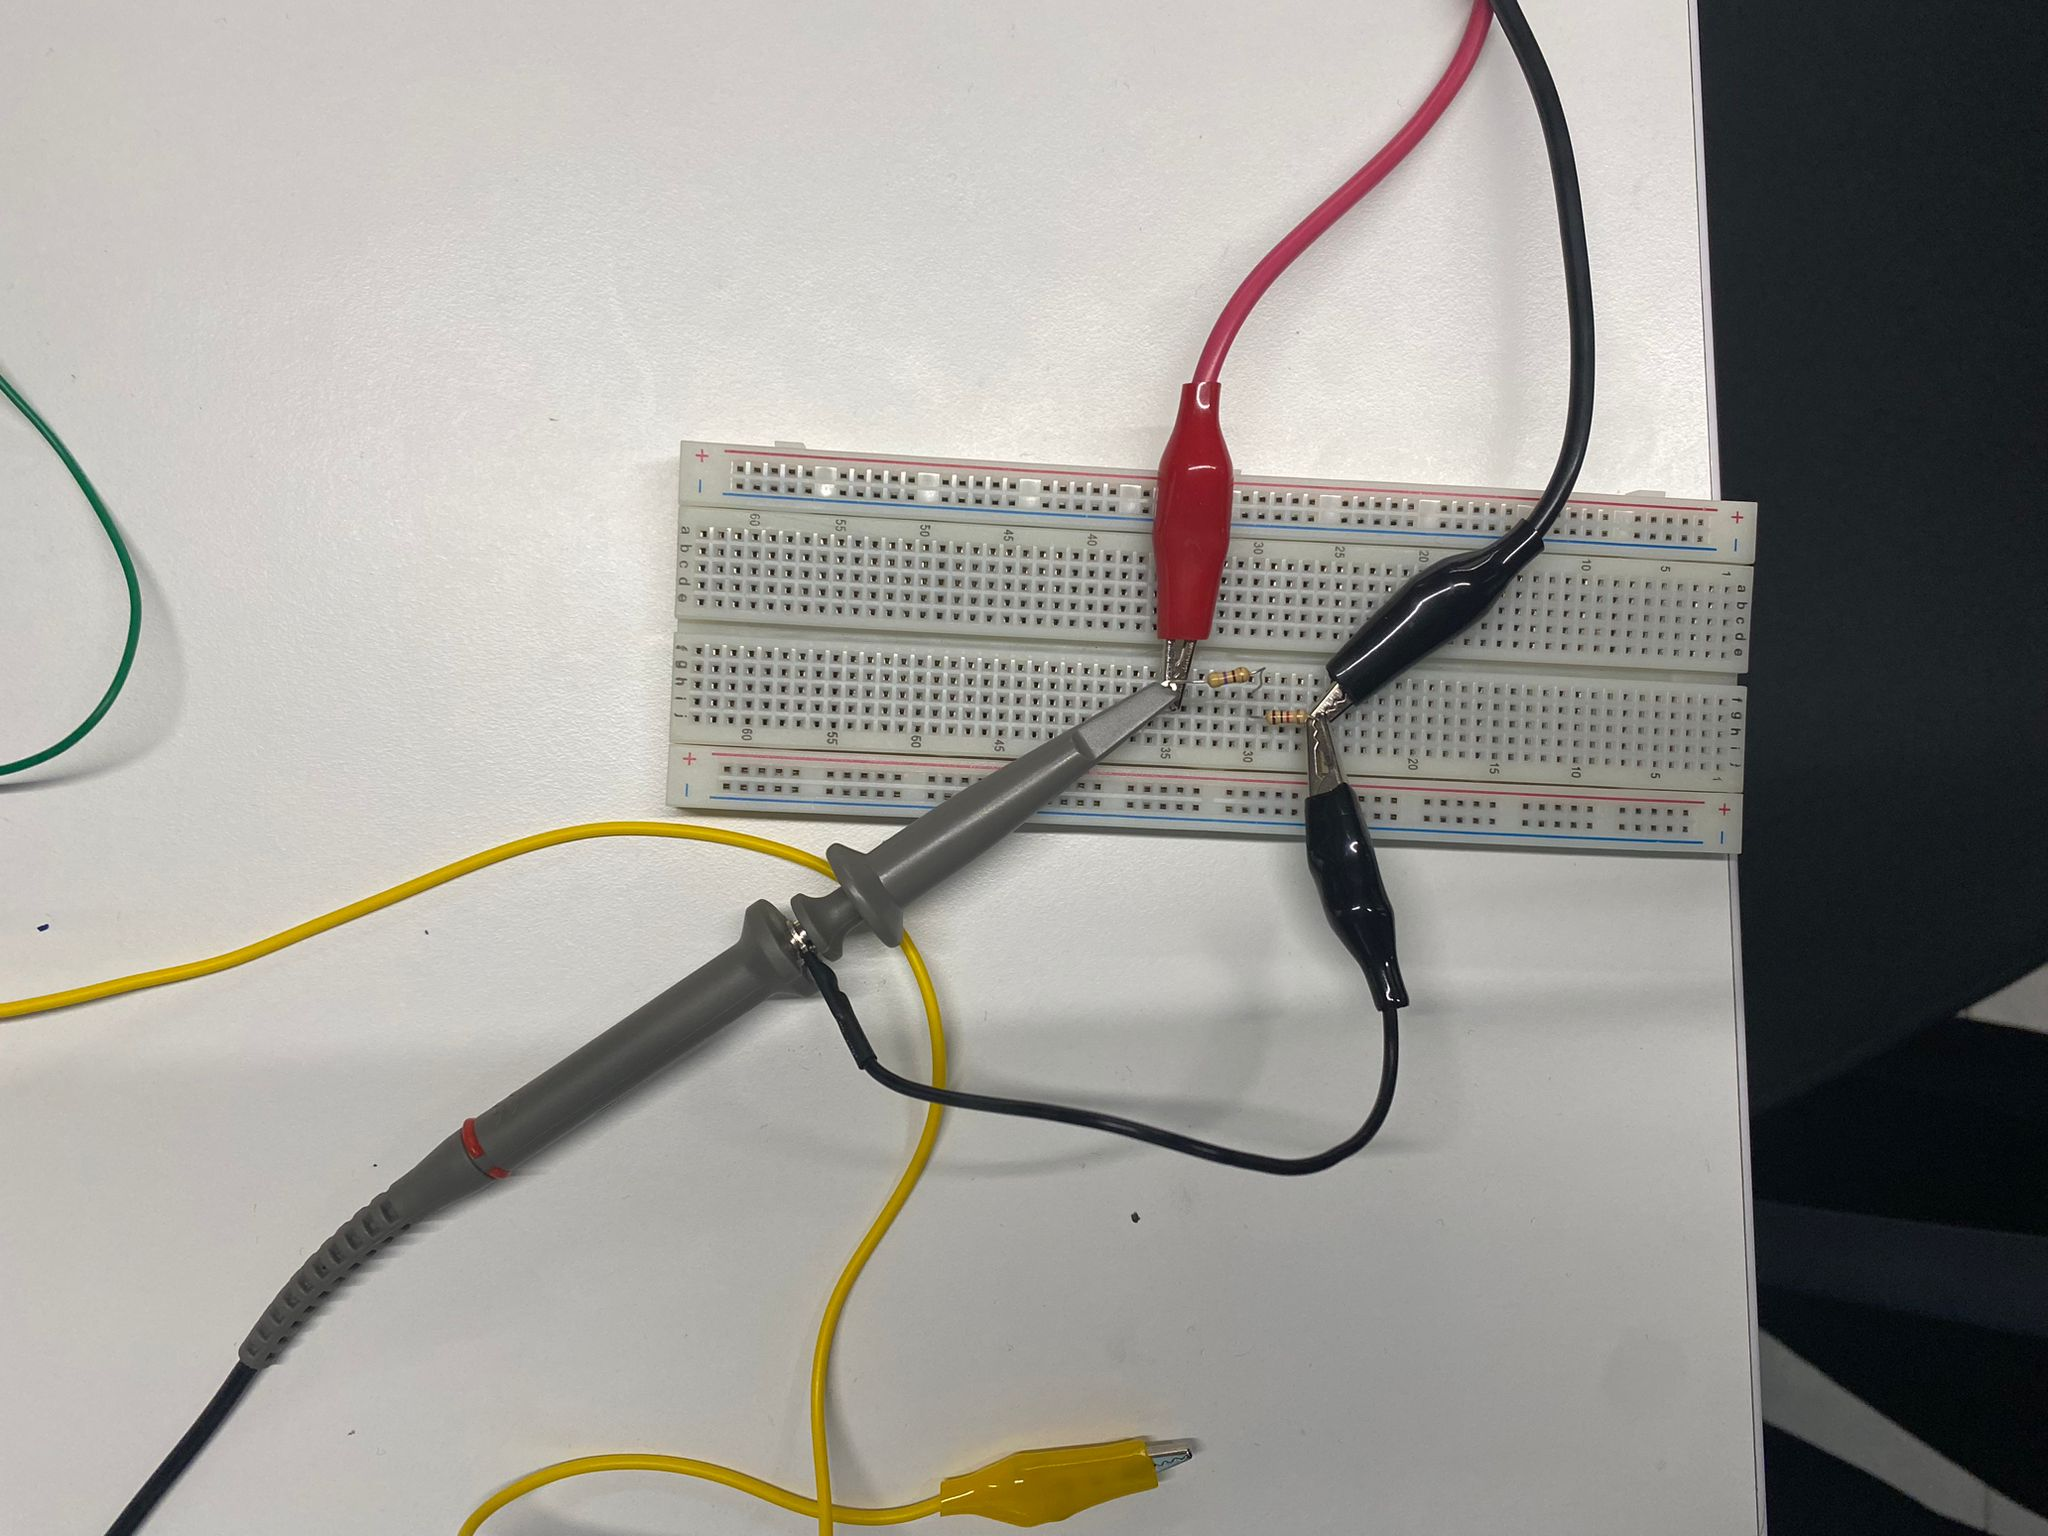
\includegraphics[width=.9\linewidth]{assets/IMG-20240307-WA0018.jpg}
            \captionof{figure}{Circuit Connection on Breadboard}
            \label{breadboard-circuit-connection}
        \end{minipage}%
        \begin{minipage}{.5\textwidth}
            \centering
            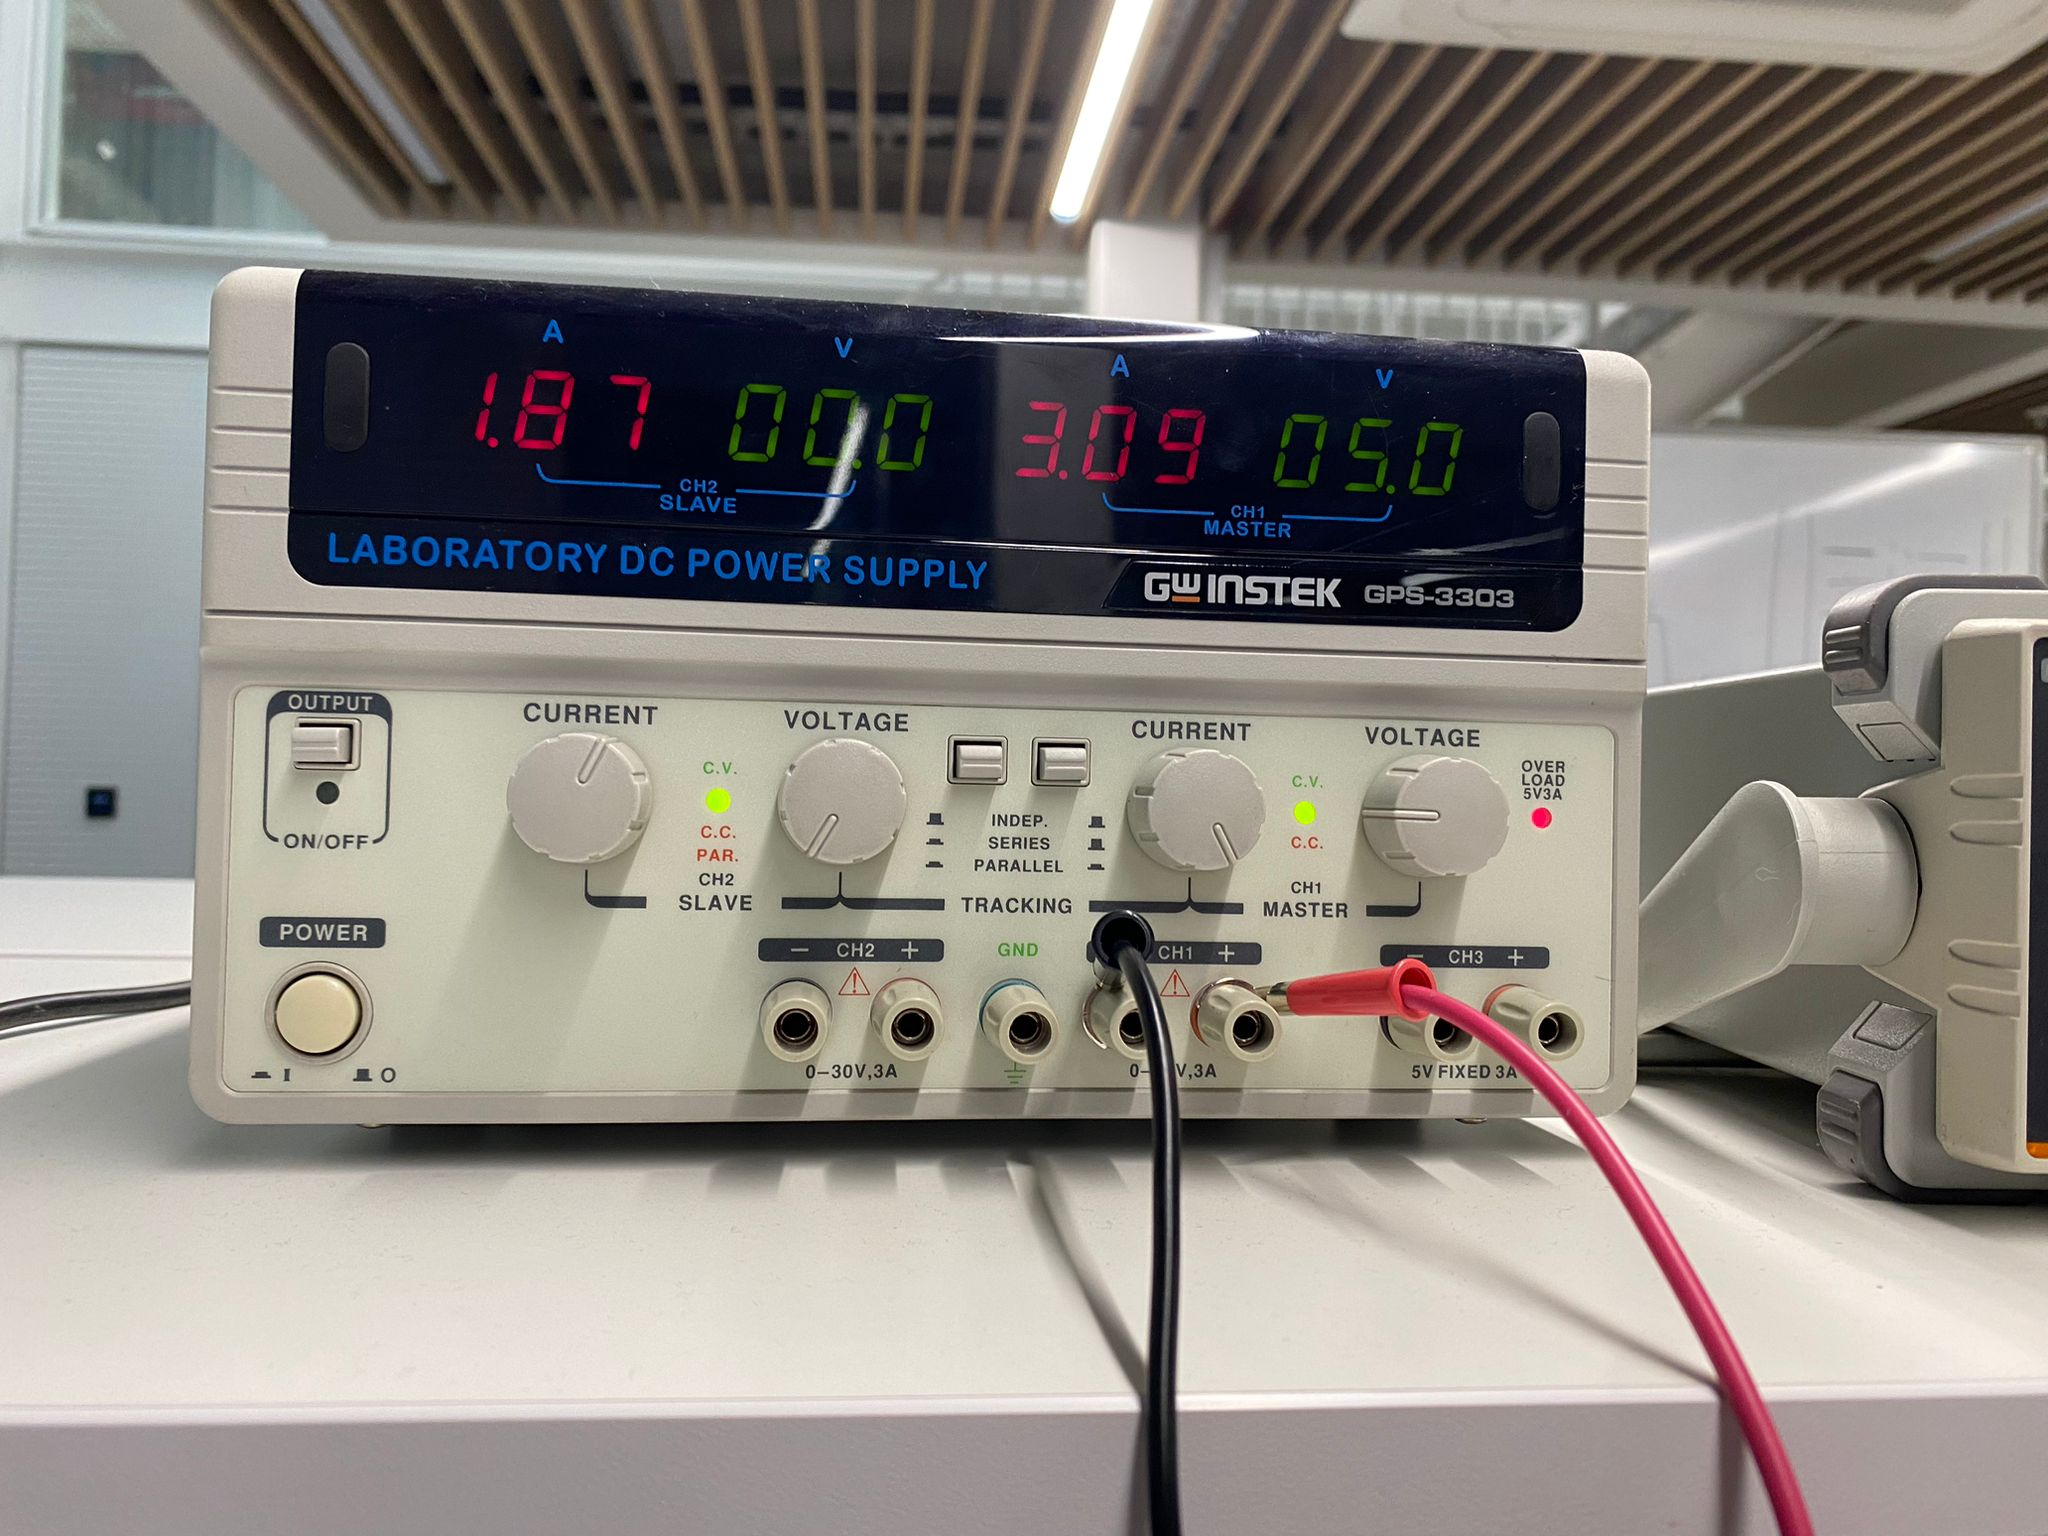
\includegraphics[width=.9\linewidth]{assets/IMG-20240307-WA0012.jpg}
            \captionof{figure}{Power Supply Connection}
        \end{minipage}
    \end{figure}

    \newpage
    \thispagestyle{plain}

    \item We have measured the current values and these are the results:
    \begin{figure}[h]
        \centering
        \begin{minipage}{0.75\textwidth}
            \includegraphics[width=1\linewidth]{assets/series-measurement.png}
            \caption{Experimental Measurements of the Series Circuit}
            \label{current-measurements}
        \end{minipage}
    \end{figure}
    \begin{figure}[h]
        \centering
        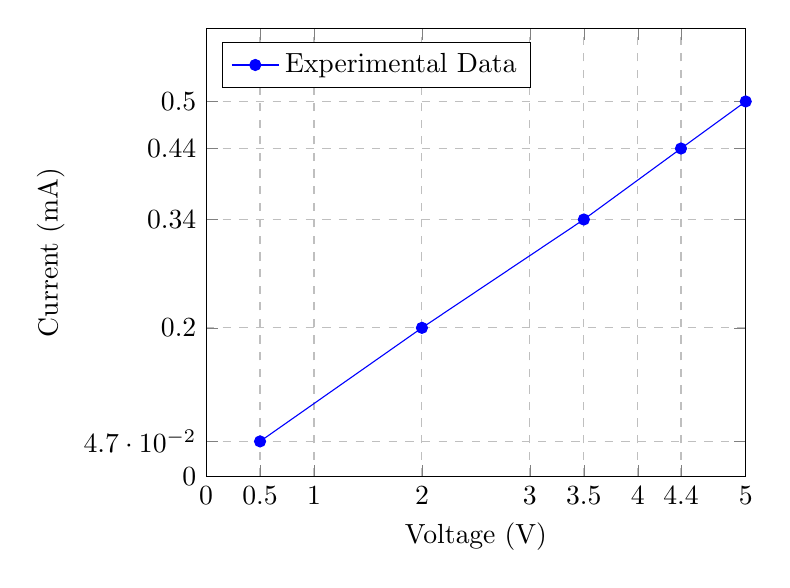
\begin{tikzpicture}
            \begin{axis}[
                xlabel={Voltage (V)},
                ylabel={Current (mA)},
                xmin=0, xmax=5,
                ymin=0, ymax=0.6,
                xtick={0, 0.5, 1, 2, 3, 3.5, 4, 4.4, 5},
                ytick={0, 0.047, 0.199, 0.344, 0.439, 0.502, 1},
                legend pos=north west,
                ymajorgrids=true,
                xmajorgrids=true,
                grid style=dashed,
            ]
                \addplot[
                    color=blue,
                    mark=*,
                ]
                coordinates {
                    (0.5, 0.047)
                    (2, 0.199)
                    (3.5, 0.344)
                    (4.4, 0.439)
                    (5, 0.502)
                };
                \legend{Experimental Data}
            \end{axis}
        \end{tikzpicture}
        \caption{Voltage-Current Graph of the Experimental Circuit According to the Figure\#\ref{current-measurements}}
    \end{figure}
    
    \newpage
    \thispagestyle{plain}

    \item We have compared the theoretical and experimental results and these are the results:
    \begin{figure}[h]
        \centering
        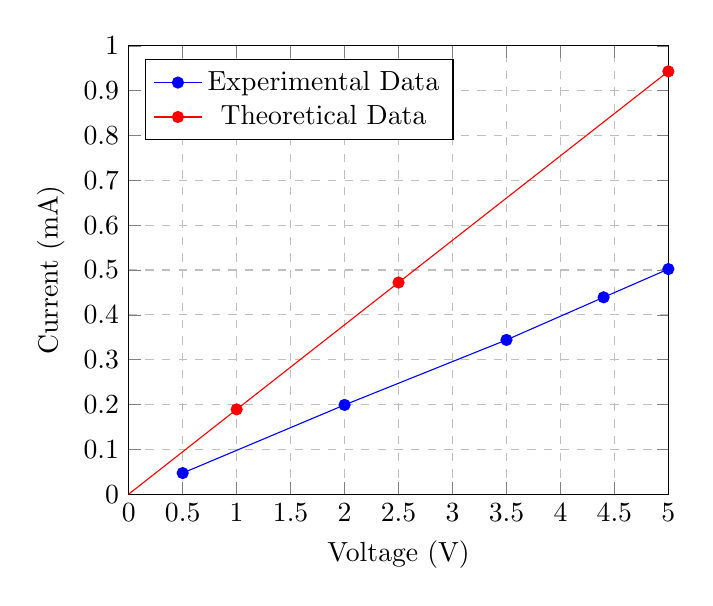
\begin{tikzpicture}
            \begin{axis}[
                xlabel={Voltage (V)},
                ylabel={Current (mA)},
                xmin=0, xmax=5,
                ymin=0, ymax=1,
                xtick={0, 0.5, 1, 1.5, 2, 2.5, 3, 3.5, 4, 4.5, 5},
                ytick={0, 0.1, 0.2, 0.3, 0.4, 0.5, 0.6, 0.7, 0.8, 0.9, 1},
                legend pos=north west,
                ymajorgrids=true,
                xmajorgrids=true,
                grid style=dashed,
            ]
                \addplot[
                    color=blue,
                    mark=*,
                ]
                coordinates {
                    (0.5, 0.047)
                    (2, 0.199)
                    (3.5, 0.344)
                    (4.4, 0.439)
                    (5, 0.502)
                };
                \addlegendentry{Experimental Data}

                \addplot[
                    color=red,
                    mark=*,
                ]
                coordinates {
                    (-5, -0.943)
                    (-1, -0.189)
                    (1, 0.189)
                    (2.5, 0.472)
                    (5, 0.943)
                };
                \addlegendentry{Theoretical Data}
            \end{axis}
        \end{tikzpicture}
        \caption{Voltage-Current Graph Comparasion}
    \end{figure}
\end{enumerate}

\subsection{Results}
We have measured the voltage and current values of the series circuit and compared the results with the theoretical values. The results are close to the theoretical values. The differences between the theoretical and experimental values are due to the tolerance of the resistors and the measurement errors.

\newpage
\thispagestyle{plain}
